\section{Experiments}

\subsection{Experimental Setup}

\paragraph{Datasets.} We use AMOS~\citep{ji2022amos} (240 training, 60 validation CT volumes, 13 abdominal organs, resampled to 1.5mm isotropic, $128^3$ crops) as the primary dataset and BTCV~\citep{landman2015btcv} (21 training, 9 validation, 13 organs) for external validation. Both datasets provide multi-organ annotations enabling paired prompt sampling.

\paragraph{Model and Adaptation.} SAM-Med3D-turbo~\citep{wang2023sam_med3d} with frozen ViT-B image encoder. LoRA adaptation (rank=8) on prompt encoder and mask decoder, yielding 1.9M trainable parameters (1.89\% of 100.5M total).

\paragraph{Training.} 50 epochs, AdamW optimizer (LR $10^{-4}$, weight decay 0.01), 2-epoch linear warmup followed by cosine decay to $10^{-6}$, batch size 1 with gradient accumulation 4. Three random seeds (42, 123, 7) for main experiments. Checkpoint selection: maximum validation Dice subject to Switch Accuracy $\geq$ 0.90.

\paragraph{Evaluation Protocol.} We construct a fixed prompt bank of 514 paired prompts (deterministic across all methods) to ensure fair comparison. Each pair consists of two point prompts targeting different organs in the same volume. We report Dice score and Switch Accuracy with McNemar test for statistical significance ($p < 0.001$).

\paragraph{Baselines.} (1) \textbf{Frozen}: SAM-Med3D without adaptation; (2) \textbf{seg-only}: LoRA fine-tuning with standard Dice+BCE loss, single prompt per step; (3) \textbf{Ours}: Paired Prompt-Contrastive Training with full loss (Eq.~\ref{eq:total_loss}).

\subsection{Main Results}

Table~\ref{tab:main} presents the main comparison on AMOS (3 seeds) and BTCV (external validation).

\begin{table}[t]
\centering
\small
\caption{Main results on AMOS and BTCV. Our method achieves near-perfect Switch Accuracy with modest Dice cost. McNemar test: $p < 0.001$ for Switch improvement across all seeds.}
\label{tab:main}
\begin{tabular}{lcc}
\toprule
\textbf{Method} & \textbf{Dice} & \textbf{Switch Acc.} \\
\midrule
\multicolumn{3}{l}{\textit{AMOS (3 seeds, mean $\pm$ std)}} \\
Frozen SAM-Med3D & 0.450 & 0.208 \\
seg-only (LoRA) & 0.720$\pm$0.006 & 0.483$\pm$0.037 \\
\textbf{Ours (Paired)} & \textbf{0.676$\pm$0.006} & \textbf{0.993$\pm$0.012} \\
\midrule
\multicolumn{3}{l}{\textit{BTCV (external validation)}} \\
seg-only (LoRA) & 0.745 & 0.312 \\
\textbf{Ours (Paired)} & \textbf{0.704} & \textbf{1.000} \\
\bottomrule
\end{tabular}
\end{table}

Standard fine-tuning (seg-only) improves Dice substantially (0.450$\to$0.720) but Switch Accuracy only reaches 0.483---the model still ignores prompts nearly half the time. Our method achieves Switch Accuracy 0.993 (+51.0 points over seg-only) with a 4.4-point Dice cost. The Dice gap is modest and expected: some segmentation capacity is redirected toward prompt-conditioned behavior rather than unconditional organ prediction.

On BTCV external validation, the improvement is even larger: Switch 1.000 vs 0.312 (+68.8 points), demonstrating strong generalization. The consistent pattern across datasets confirms that paired training fundamentally changes model behavior rather than overfitting to dataset-specific patterns.

\subsection{Training Dynamics}

Figure~\ref{fig:curves} shows Dice and Switch Accuracy over 50 training epochs. The seg-only baseline exhibits a characteristic pattern: Dice climbs steadily while Switch Accuracy fluctuates around 0.5 without improvement---the model learns better segmentation but not better prompt following. In contrast, our method maintains Switch Accuracy above 0.95 from epoch 1 onward while Dice gradually improves, demonstrating that paired training establishes prompt faithfulness immediately and maintains it throughout optimization.

\begin{figure}[t]
\centering
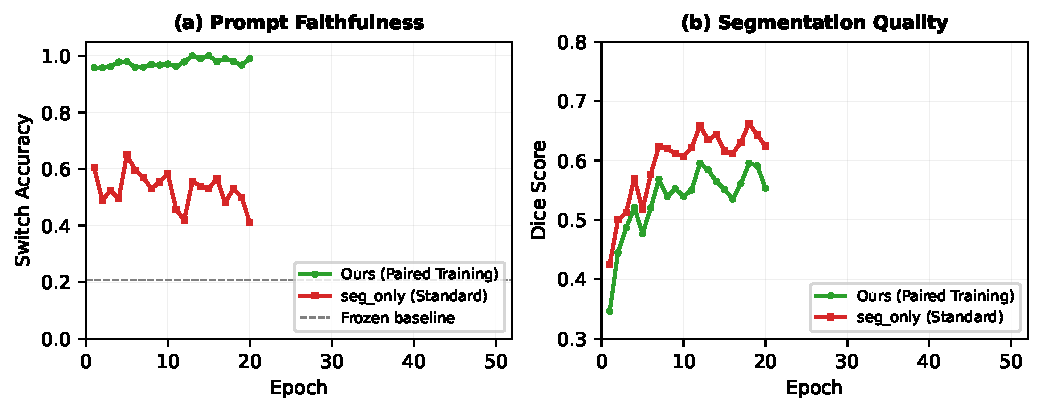
\includegraphics[width=\columnwidth]{figures/fig3_training_curves.pdf}
\caption{Training dynamics over 50 epochs. (a) Switch Accuracy: our method maintains $>$0.95 throughout while seg-only stagnates at $\sim$0.5. (b) Dice: both methods improve, with seg-only reaching slightly higher final Dice due to unconstrained optimization.}
\label{fig:curves}
\end{figure}

\subsection{Mechanism Ablation}
\label{sec:mechanism}

To isolate the contribution of each component, we conduct a factor-isolation experiment (Table~\ref{tab:ablation}, 20 epochs, seed=42). We vary two binary factors---paired vs.\ single prompt training, and presence vs.\ absence of auxiliary losses---to determine what drives faithfulness. All configurations use identical training budgets: same number of optimizer steps, same images per epoch, and same LoRA parameters. Paired methods process two decoder passes per image (reusing the cached encoder embedding), while single-prompt methods process one. This means paired methods see twice as many prompt-target supervision signals per step; however, the seg-only baseline trained for equivalent total prompt exposures (100 epochs) still achieves only Switch 0.55, confirming that exposure alone is insufficient without simultaneous pairing.

\begin{table}[t]
\centering
\small
\caption{Mechanism ablation (20 epochs, AMOS). Paired training is the dominant factor (+40pt Switch). Grounding without paired training is counterproductive.}
\label{tab:ablation}
\begin{tabular}{lccc}
\toprule
\textbf{Method} & \textbf{Paired} & \textbf{Sw. Acc} & \textbf{Dice} \\
\midrule
seg-only & No & 0.55 & 0.62 \\
+ grounding only & No & 0.43 & 0.62 \\
\midrule
paired (seg only) & Yes & 0.94 & 0.60 \\
+ grounding & Yes & 0.99 & 0.57 \\
+ ground + switch & Yes & 0.99 & 0.60 \\
\bottomrule
\end{tabular}
\end{table}

The results reveal a clear hierarchy of importance:

\textbf{Paired training is necessary and sufficient} (+40 points). Moving from single-prompt to paired-prompt training---even without any auxiliary loss---jumps Switch Accuracy from 0.55 to 0.94. This is the dominant mechanism.

\textbf{Grounding adds marginal benefit on top of paired training} (+5 points, 0.94$\to$0.99). However, grounding \emph{without} paired training actually \emph{decreases} Switch Accuracy (0.55$\to$0.43). This counterintuitive result suggests that grounding reinforces the model tendency to predict based on spatial priors without learning to differentiate between prompts.

\textbf{Switch margin loss adds negligible benefit} (0.99$\to$0.99). When paired training already provides the contrastive signal, the explicit margin loss is redundant.

Figure~\ref{fig:ablation} visualizes this hierarchy, making clear that the contribution is a \emph{training paradigm} (paired exposure), not a specific loss function.

\begin{figure}[t]
\centering
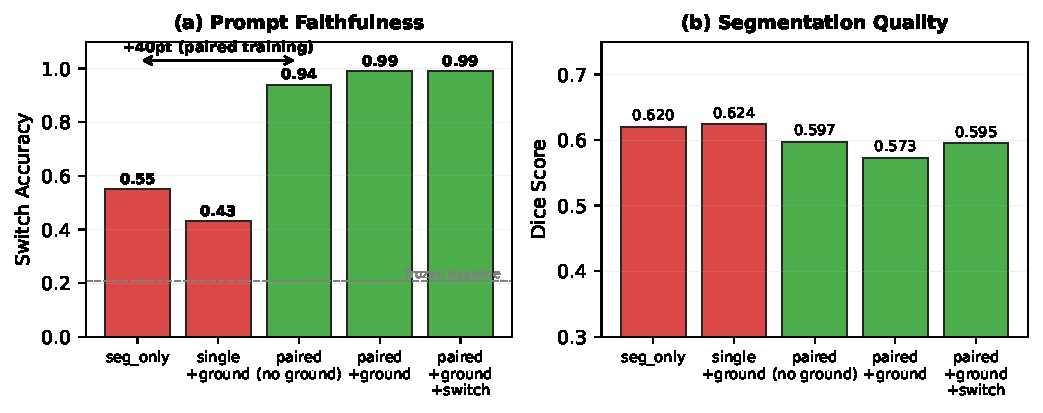
\includegraphics[width=\columnwidth]{figures/fig5_mechanism_ablation.pdf}
\caption{Mechanism ablation visualization. Single-prompt methods (red) fail regardless of loss design. Paired-prompt methods (green) succeed regardless of auxiliary losses. The gap between groups ($\sim$40 points) dwarfs within-group variation.}
\label{fig:ablation}
\end{figure}

\subsection{Hyperparameter Robustness}

Table~\ref{tab:robust} demonstrates that all paired-training configurations maintain Switch Accuracy $\geq$0.978 across a wide range of margin values and loss weights.

\begin{table}[t]
\centering
\small
\caption{Hyperparameter robustness (20 epochs, AMOS). All paired-training configurations maintain Switch $\geq$0.978.}
\label{tab:robust}
\begin{tabular}{lcc}
\toprule
\textbf{Configuration} & \textbf{Switch Acc.} & \textbf{Dice} \\
\midrule
margin = 0.1 & 0.990 & 0.561 \\
margin = 0.2 (default) & 0.990 & 0.595 \\
margin = 0.3 & 0.990 & 0.555 \\
\midrule
$\lambda_{\text{switch}}$ = 0.25 & 0.989 & 0.567 \\
$\lambda_{\text{switch}}$ = 1.0 (default) & 0.990 & 0.595 \\
$\lambda_{\text{switch}}$ = 2.0 & 0.990 & 0.545 \\
\bottomrule
\end{tabular}
\end{table}

The Dice score varies modestly with $\lambda_{\text{switch}}$ (0.545--0.595), suggesting a mild tradeoff: higher switch weight slightly reduces segmentation accuracy. However, Switch Accuracy remains near-perfect across all settings, indicating that the paired training mechanism is inherently robust and does not require careful tuning.

\subsection{Cross-Domain Analysis}

To assess whether prompt unfaithfulness is specific to 3D medical SAM, we evaluate SAM2~\citep{ravi2024sam2} on COCO natural images using the same Switch Accuracy protocol. SAM2 achieves 0.954 Switch Accuracy out of the box. While direct comparison is limited by differences in model scale, training data, and modality, this result suggests that prompt unfaithfulness is not inherent to the promptable segmentation paradigm but rather emerges under the specific conditions of 3D medical adaptation.

We hypothesize this specificity arises from two factors: (1) limited diversity in medical training data (anatomical structures are highly consistent across patients), enabling the model to exploit spatial priors; and (2) the frozen encoder paradigm, where only the decoder is adapted, limiting the model capacity to learn new prompt-conditioned features.

\subsection{Qualitative Results}

Figure~\ref{fig:qualitative} shows representative examples comparing seg-only and our method. When given two different organ prompts on the same image, seg-only produces nearly identical predictions (both targeting the dominant organ), while our method correctly switches the segmentation target to match each prompt.

\begin{figure}[t]
\centering
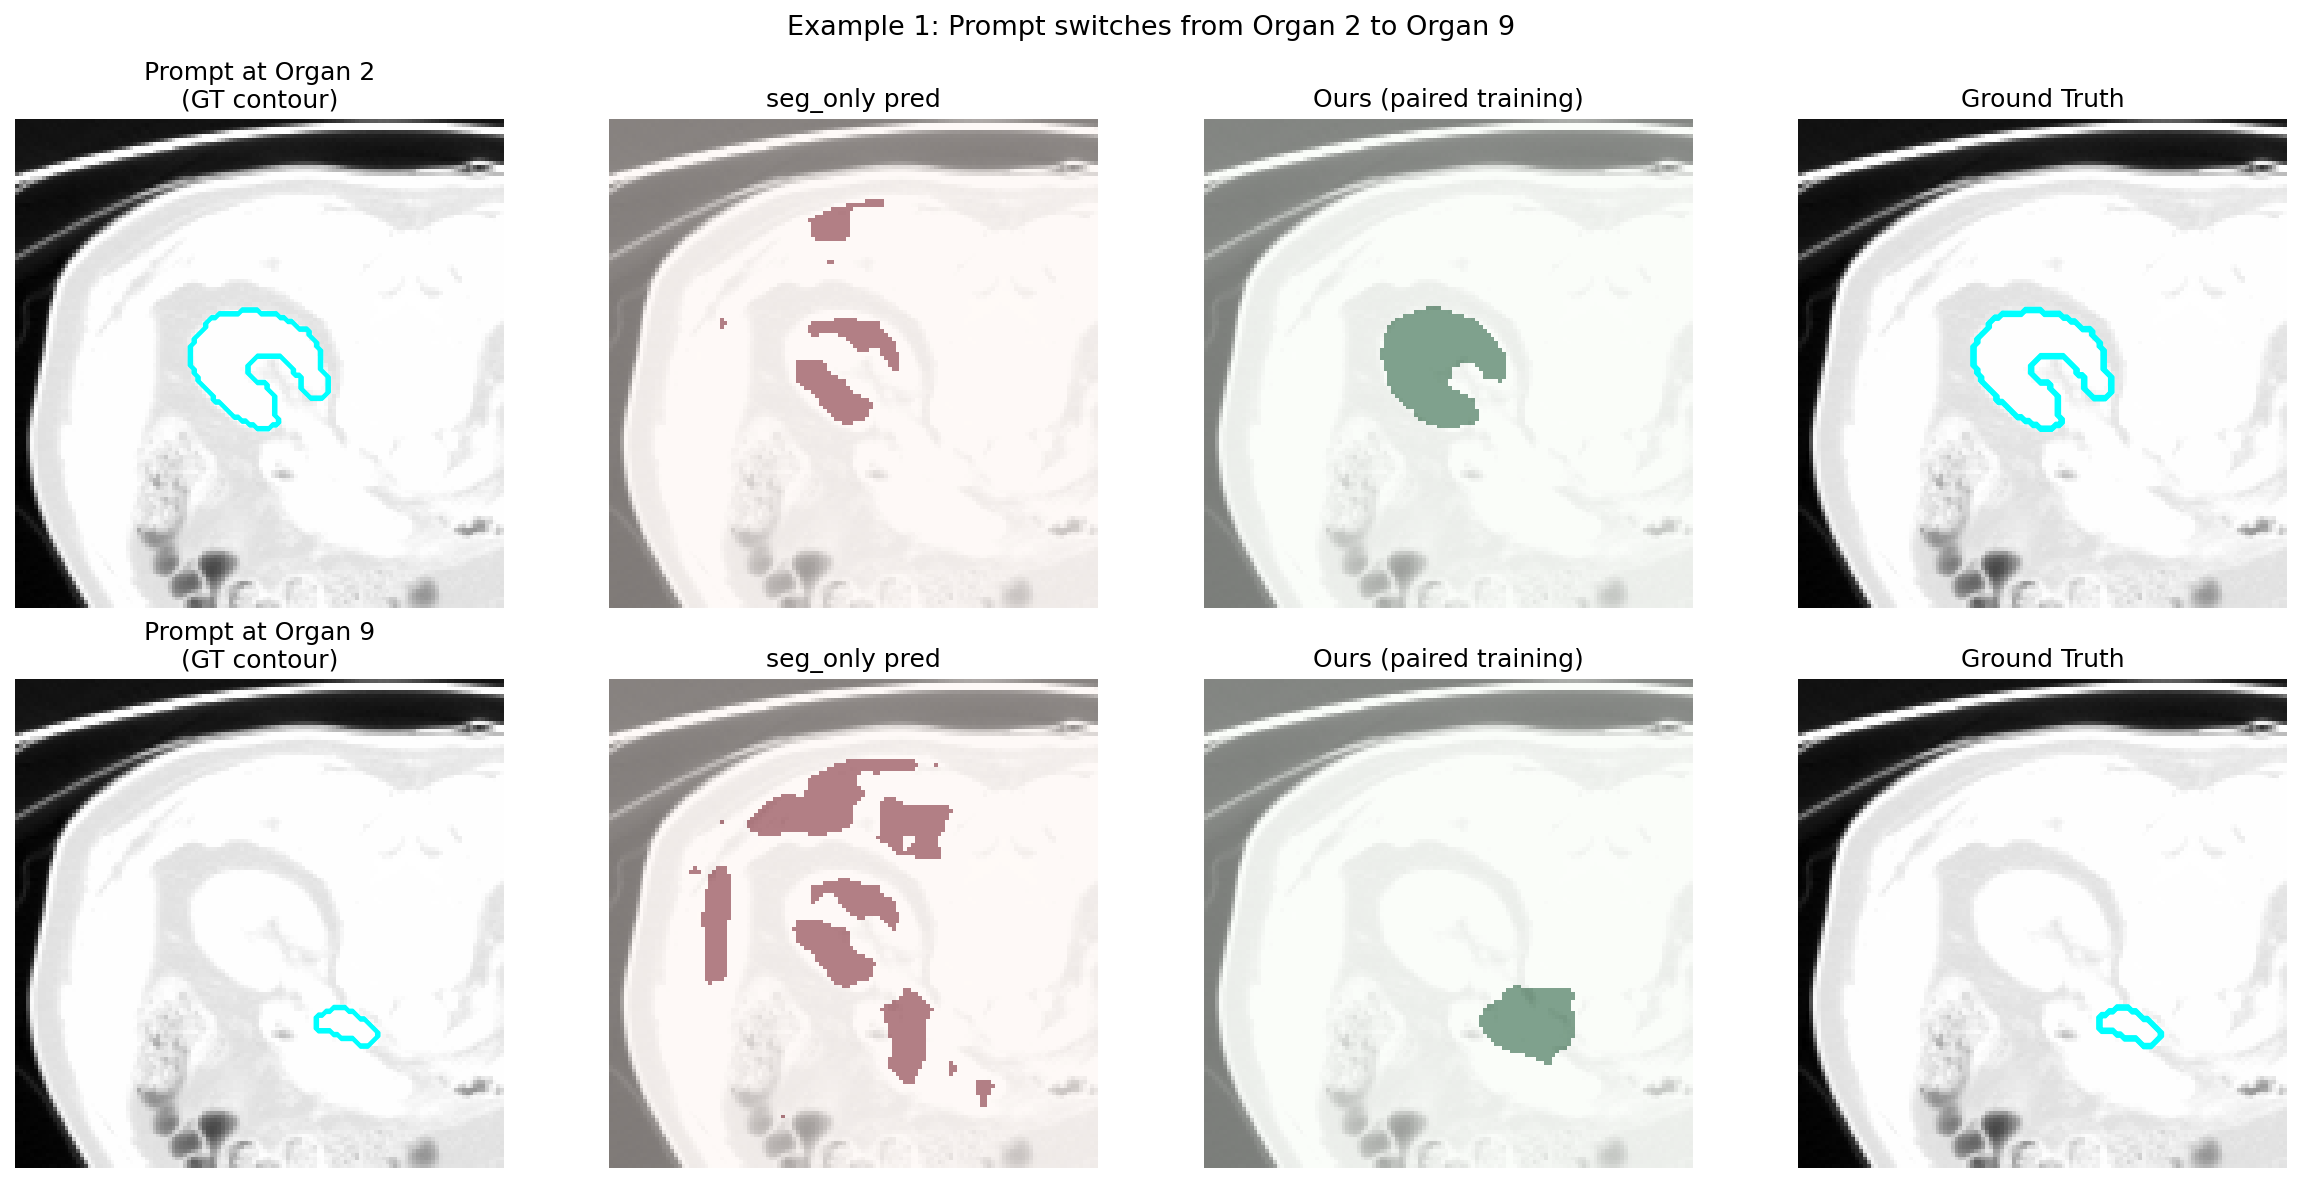
\includegraphics[width=\columnwidth]{figures/fig4_qualitative.png}
\caption{Qualitative comparison. Each row shows predictions for a different prompt target on the same image. seg-only produces identical outputs regardless of prompt (unfaithful). Our method correctly segments the prompted organ (faithful).}
\label{fig:qualitative}
\end{figure}
